% Chapter Template

\chapter{Testing The Drift Diffusion Solver} % Main chapter title

\label{Chapter4} % Change X to a consecutive number; for referencing this chapter elsewhere, use \ref{ChapterX}

\lhead{Chapter 4. \emph{Testing Drift Diffusion Solver}} % Change X to a consecutive number; this is for the header on each page - perhaps a shortened title

\begin{doublespace}

The past chapter shows the details of how to solve drift-diffusion and Poisson's equation using finite difference method. In this chapter steady state and transient analysis for drift diffusion equations using finite difference is compared to analytical solutions as well as a commercially available simulator called 'COMSOL Multiphysics' which uses finite element method instead of a finite difference approach. The following test cases were made to ensure that the key parts of the finite difference scheme run properly and produce accurate results. 

\section{Solution for Closed Boundary}
In this section the accuracy of the finite difference solution in steady state is tested. In order to do this, a simple 1-D problem with a finite number of negatively charged particles over a certain distance subject to constant electric field is used. This is the same problem that is solved analytically in section 3.3.1. It is also assumed that the charge density is very low and does not affect the electric field. Both ends of the simulation domain have no flow boundary conditions for charged particles. The solution process requires an initial distribution for the charge density over the area. For this problem the density of the negative particles was initialized to be uniform over the entire region. 

Since the differential equations are uncoupled solving Poisson's equation only once is sufficient to determine the electric field over the course of the entire simulation. Figures \ref{5E} and \ref{5pot} show the potential and the electric field distribution over the entire simulation area calculated from Poisson's equation using finite difference. 

\begin{figure}
\centering
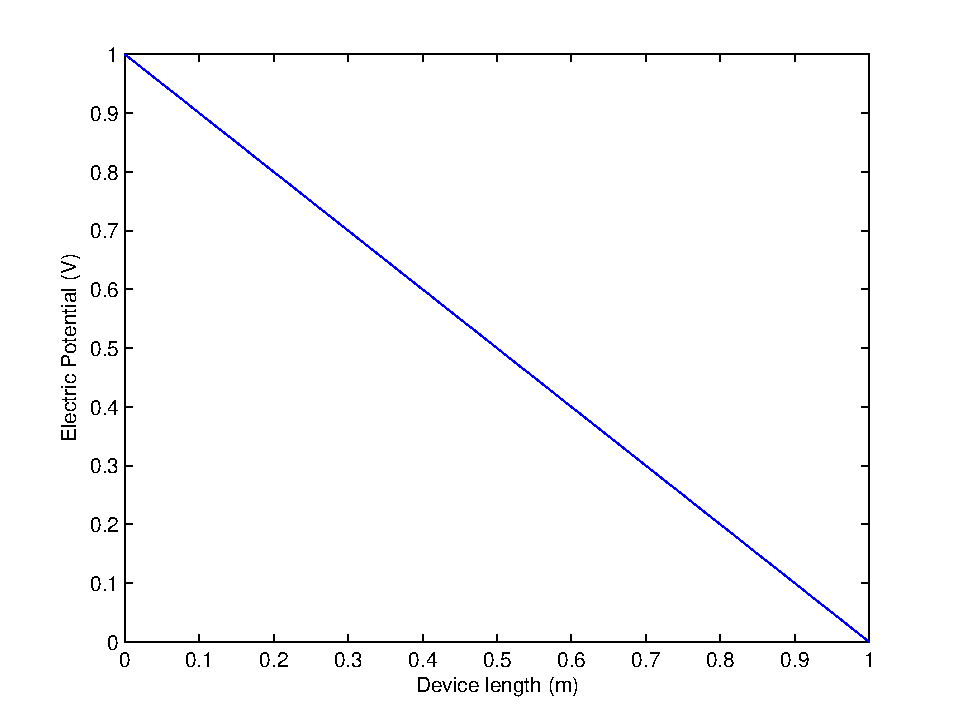
\includegraphics[scale=0.65]{5101}
\caption{Potential Distribution} 
\label{5pot}
\end{figure}

\begin{figure}
\centering
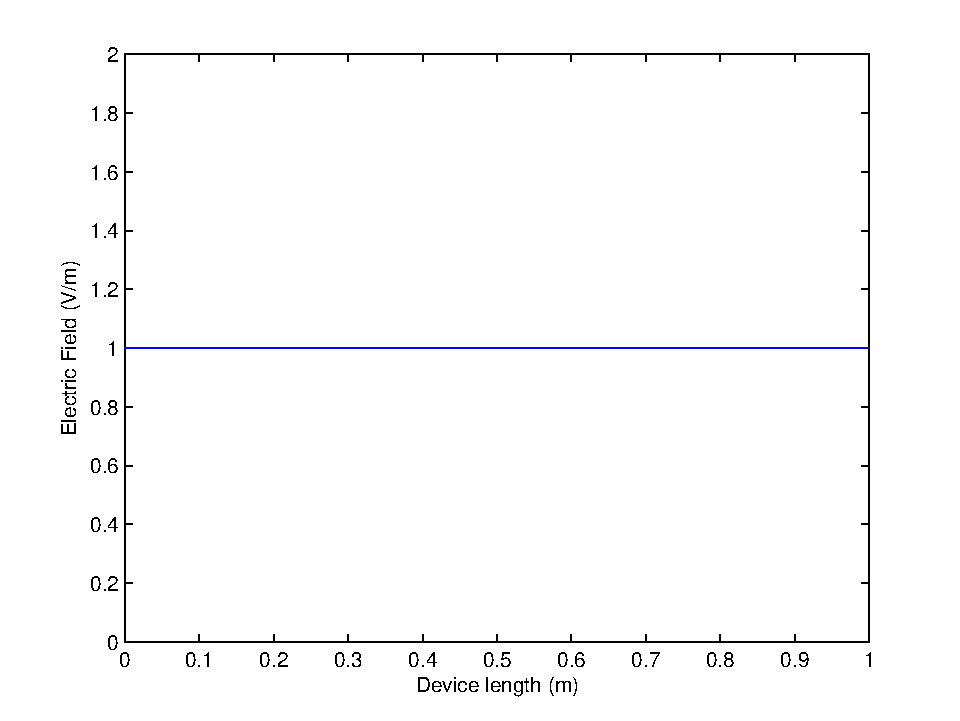
\includegraphics[scale=0.65]{5102}
\caption{Electric Field Distribution} 
\label{5E}
\end{figure}

\clearpage

Figure  \ref{5ss} has two simulation results as well as the exact solution of this problem. The green line represents the result given by the finite difference method at steady state. It can be seen from the graph that the steady state solution generated by both COMSOL and finite difference matched the analytical solution.

\begin{figure}
\centering
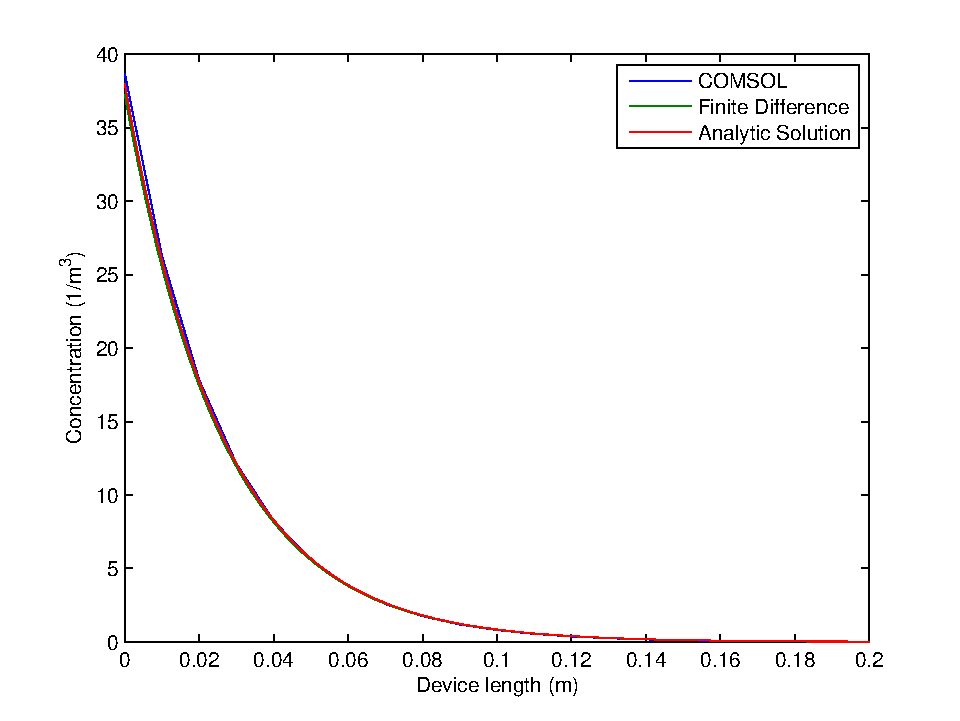
\includegraphics[scale=0.8]{511}
\caption{Steady State Negative Charge Density} 
\label{5ss}
\end{figure}

\begin{figure}[!htp]
\centering
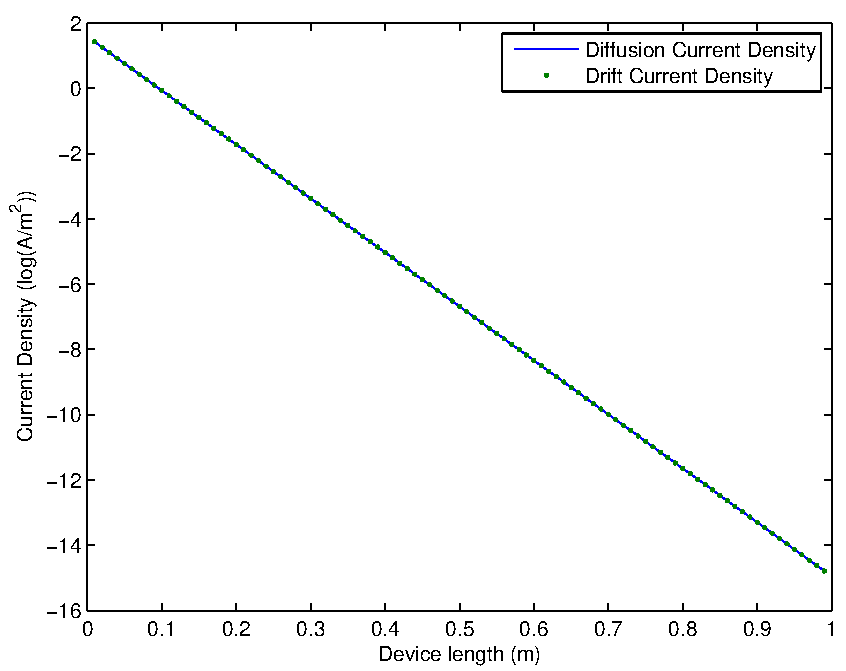
\includegraphics[scale=0.8]{513}
\caption{Finite Difference Drift and Diffusion Current Densities}
 \label{5curdens}
\end{figure}

While deriving an analytical solution for this problem it was assumed that at steady state the drift current density must be equal and opposite in magnitude to the diffusion current density. In figure \ref{5curdens}, drift and diffusion current densities are shown in log scale. Overall both currents match quite tightly.

Even though the simulation results are good for this example high electric fields due to either applied potential or high charge densities can introduce inaccuracies. If the electric field is very high then the accumulation of the charge can get very steep. The exponential accumulation requires higher mesh densities for accurate calculation.

\clearpage
\section{Solutions for Open Boundary}
Another crucial aspect of the drift-diffusion simulation is its transient response. Like the previous test case, the analytic solution can be used to test the accuracy of the transient response. Two different analytic solutions for a similar drift diffusion problems which involved infinite boundaries and a uniform electric field are shown in section 3.3.2. The only difference between two cases are their initial carrier distributions. One has a rectangular and the other one has a gaussian initial carrier distribution. The finite difference scheme does not allow simulation over an infinitely long conductor. For this test case, simulation is performed until the carrier distribution gets close to a wall.   

\begin{figure}[ht]
\centering
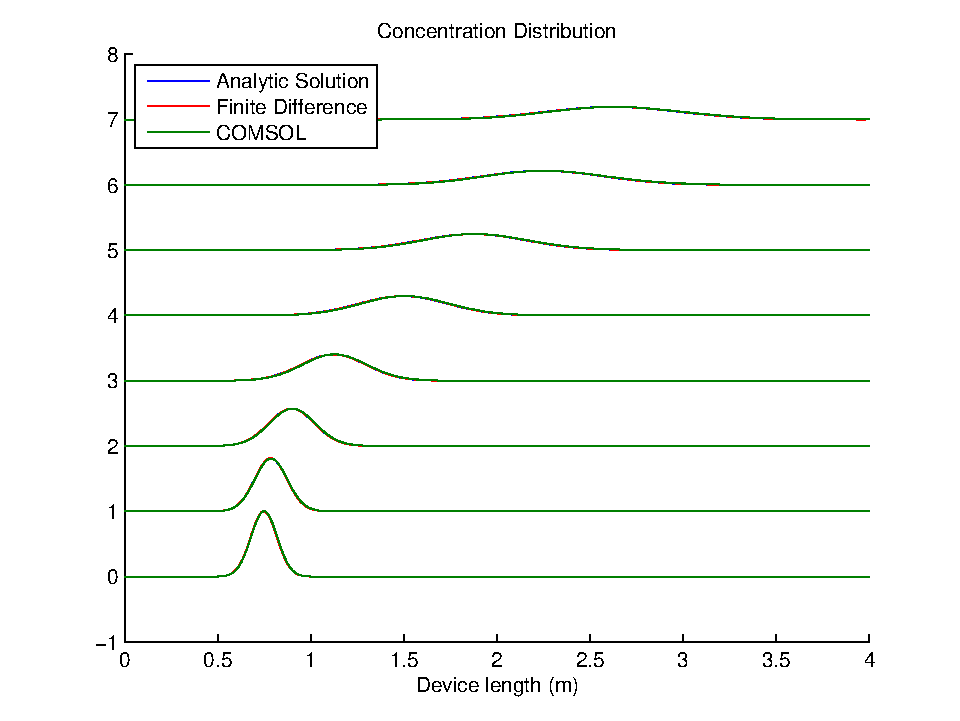
\includegraphics[scale=0.8]{5212}
\caption{Gaussian Carrier Distribution Evolving Over time} 
\label{51}
\end{figure}

Figure \ref{51} has the transient responses from COMSOL, finite difference and analytical solution. Snapshots of the carrier distributions were taken for each method at different time steps and they were superposed on top of each other. Increasing levels on the \textit{y} axis represent a carrier distributions at a different time starting from the bottom and moving forward in time towards the top. Figure \ref{51} has a gaussian initial carrier distribution. It can be seen from that the transient solution generated by both COMSOL and finite difference are quite close to the analytical solution.


\clearpage
\section{PN Junction}
In previous test cases, Poisson's equation is not coupled with drift diffusion equations. In this example both drift diffusion and Poisson's equation are tested to investigate how well they work when they are coupled together. A simple pn junction is quite adequate for this task since it has analytical solutions (under certain assumptions) for electric potential, electric field and carrier distribution.

For the simulation, initial hole and electron distributions are determined using mass action law and they are assumed to be constant at the boundaries. Keeping carrier density constant creates a mechanism in which the charge can move in and out of the simulation domain. If the charge density at any time step is higher than the fixed density then the difference will move out of the system. If there is a lack of charge at the boundary then carriers will move in to fill in the gap. Following figure (\ref{npcon}) shows the final result of bringing p and n type materials together. 
 
\begin{figure}[ht]
\centering
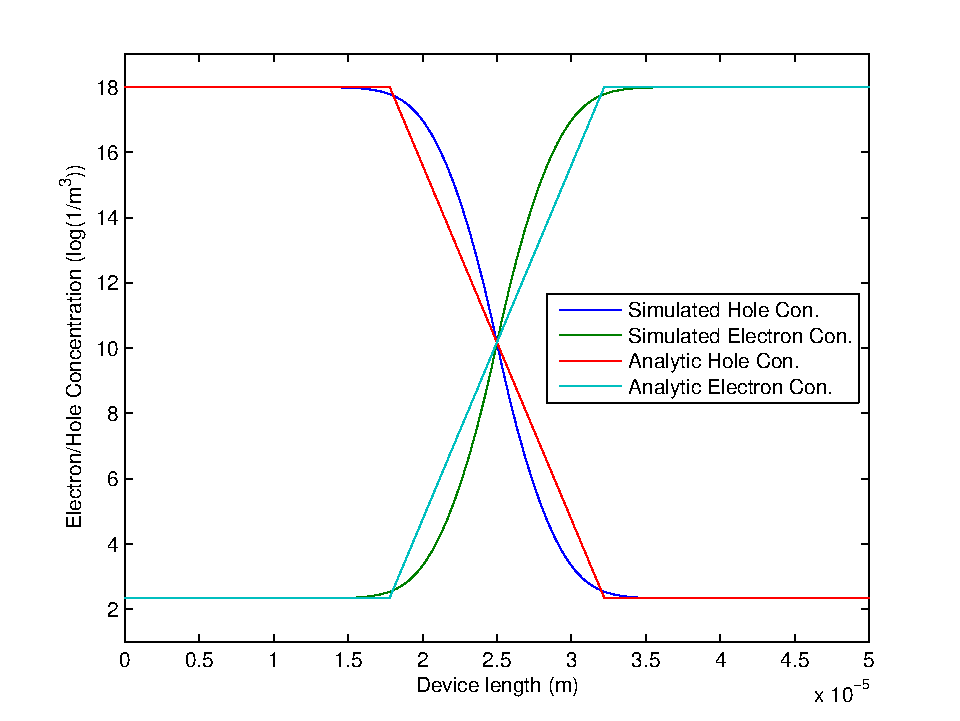
\includegraphics[scale=0.8]{5311}
\caption{Electron/hole Concentration of a PN Junction} 
\label{npcon}
\end{figure}

There is a little mismatch between simulated and analytic charge densities. Analytic solution have sharp edges and simulated solution does not. This is due to all the assumptions made in order to find an analytic solution. This mismatch can also be seen for electric field, electric potential and net charge .

 Figure \ref{pnpot} shows the potential distribution for simulated and analytic solutions. Close match in electric potential distribution shows that coupled equations can generate accurate solutions.
 
\begin{figure}[!htp]
\centering
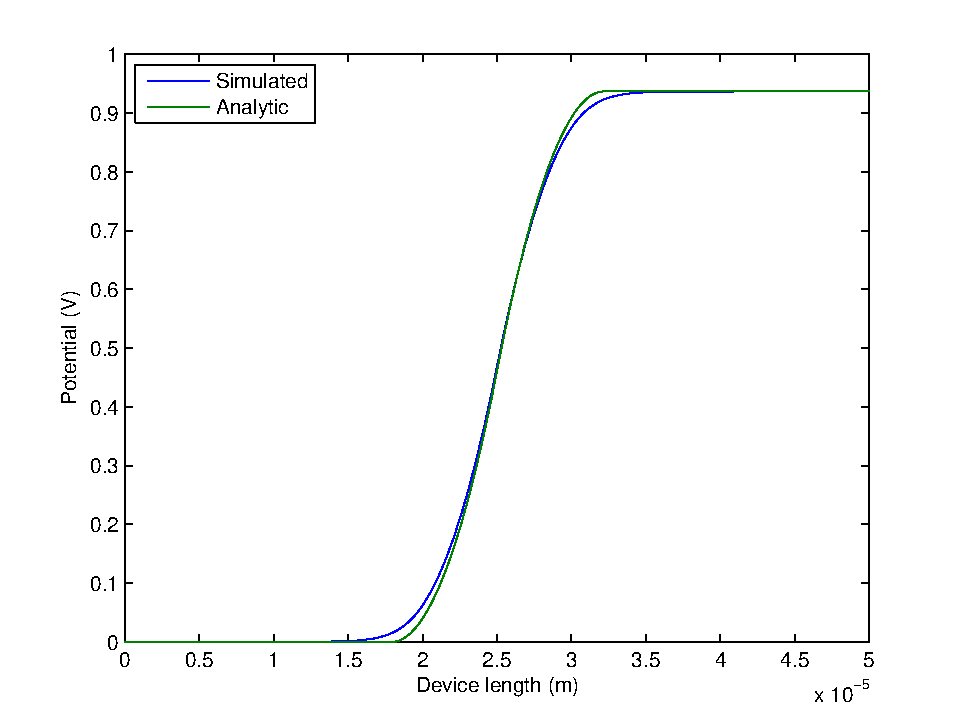
\includegraphics[scale=0.7]{5312}
\caption{Potential Distribution of a PN Junction} 
\label{pnpot}
\end{figure}

Calculation of the electric field involves one basic derivative. Since simulated potential is matching the analytic solution quite nicely the electric field should follow a similar pattern. Figure \ref{pnefield} shows that this is indeed the case, simulated electric field matches the calculated electric field.
\begin{figure}[!htp]
\centering
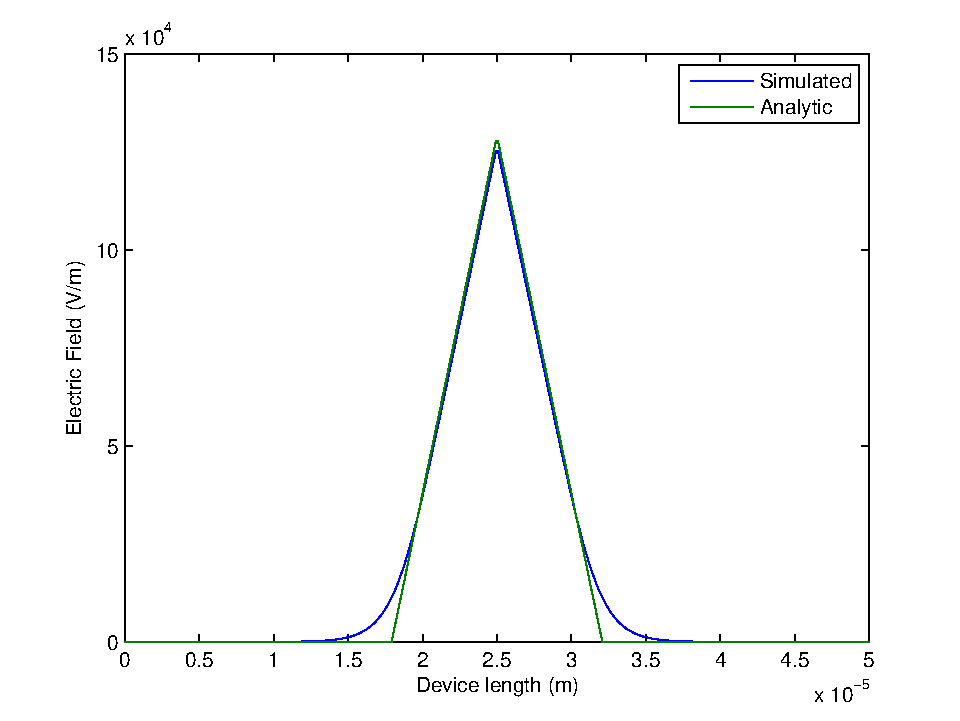
\includegraphics[scale=0.7]{5313}
\caption{Electric Field Distribution of a PN Junction} 
\label{pnefield}
\end{figure}

Figure \ref{pncd} shows the total charge distribution at steady state. Simulated net charge density follows the analytic one except the abrupt changes at two ends. 
\begin{figure}
\centering
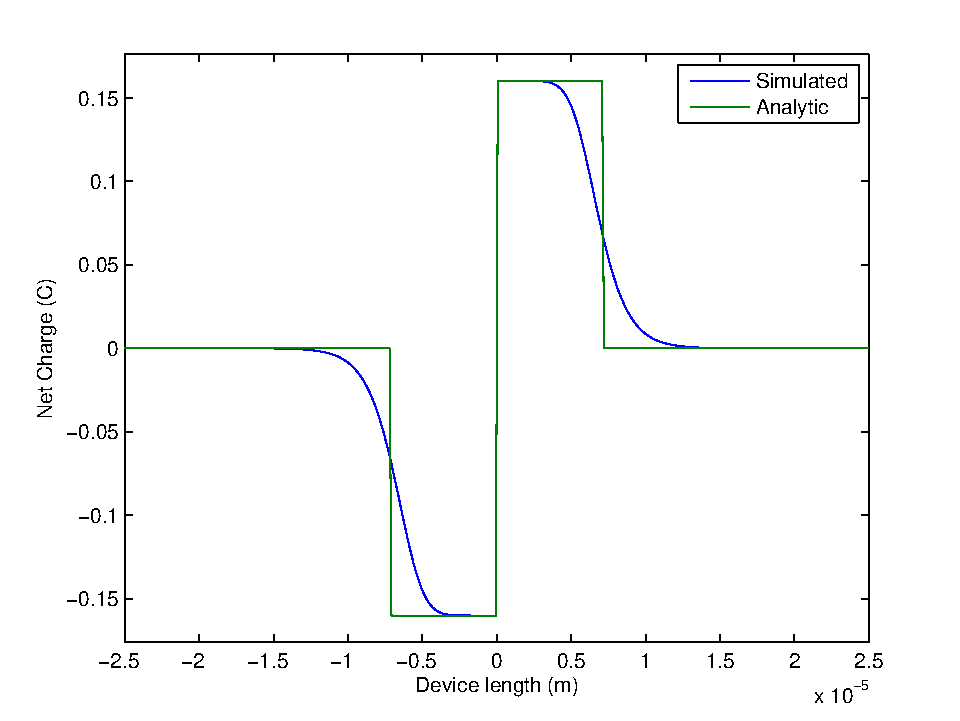
\includegraphics[scale=0.7]{5314}
\caption{Total Charge Distribution of a PN Junction} 
\label{pncd}
\end{figure}

This example showed that simulation of a system of coupled equations, drift diffusion and Poisson's equation, using finite difference can produce accurate results. This accuracy depends on the strength of the coupling. High charge densities can produce strongly coupled systems. This effect shows the importance of CFL conditions as well as the physical limitations of the simulation.


\clearpage
\section{Region Specific Particle Density Limit}

The last property of the drift diffusion simulation scheme that is tested in this section concerns the movement of lithium ions. As lithium ions move into the PEDOT:PSS they bond with PSS polymer sites and replace holes. PEDOT:PSS can only absorb lithium as long as there are available PSS polymer sites to bond with therefore PEDOT:PSS has limited capacity to accept lithium ions. This behavior is captured in the model by blocking the particle flow into an area if the density will go over a set limit. This can be achieved in two different ways. 

A soft limit can be set by making the particle mobility a function of its density. This function can be defined in such a way that it switches from a high to a low value when the particle density approaches a defined limit. This implementation is straightforward and can be used in commercial simulators but it has some drawbacks. Once the maximum particle density is reached the mobility and the diffusivity of the lithium particles are stuck at very low values. If there is an outflux of particles from that particular node then the lithium density is stuck at the limit until the mobility and the diffusivity function goes back to a value which allows more particle flow. This can introduce a considerable lag in the response of the device.  

An alternative approach is pre-calculating the particle density of a density limited node at the next time step, setting any influx to zero if the density is going to go over the limit and finally recalculating the particle densities at the next time step using the updated current densities. This mechanism sets a hard limit on the density since there is a sudden break instead of a gradual slowdown in the current flow. This density limiting mechanism is more responsive than the previous one but it requires the calculation of the next time step twice for the species that has a limit. Also a large influx of particles caused by either a big time step or a high electric field can force the algorithm to cut the current flow into a node before the density reaches its limit.

To avoid adding any lag into the system the latter method is used for the memristor simulations in this thesis. This method is implemented in the finite difference drift diffusion solver. Also a soft limit is implementend in COMSOL for comparison since it does not support the hard limit method.  

In order to test density limiting method implemented for the memristor simulation a simple example is set up. Two positively charged particles are initialized like the figure below in two separate simulations (\ref{5412}). One set of particles has a density limit of $2 \; 10^{10} \; m^{-3}$ on the right half of the simulation area and no limit on the left half. The other set has no restrictions. The initial particle density on the left half of the simulation area is set to $5 \; 10^{10} \; m^{-3}$ for both simulations.
\begin{figure}[!htp]
\centering
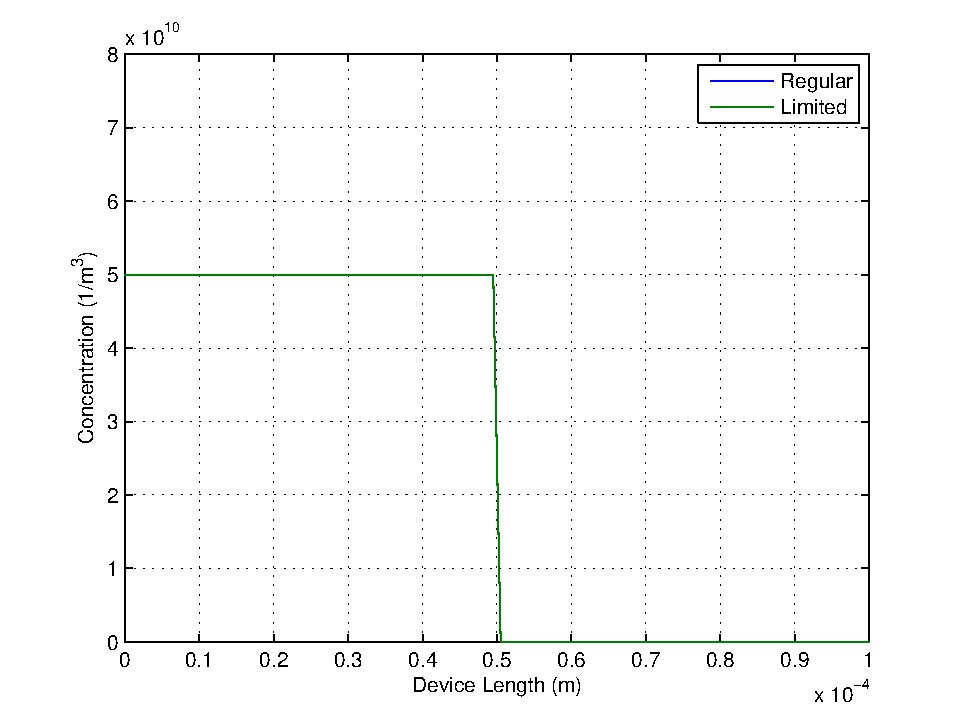
\includegraphics[scale=0.7]{5412}
\caption{Initial Particle Density} 
\label{5412}
\end{figure}

This transient simulation uses a potential pulse train. The potential is applied at the left side of the device and the right side is always grounded. For the first half of the transient simulation the applied potential is positive and for the second half it is negative. Figure \ref{5413} shows how two simulations differ when the particles are pushed towards the right wall due to the electric field created by the positive potential. Particles with no limit on the right side move freely and accumulate on the right wall. The density limit for the other particles is effectively stopping them from migrating and accumulating freely. Once the limit is reached at a certain node the density cannot increase any further and that node turns into a no flow wall. 

\begin{figure}[!htp]
\centering
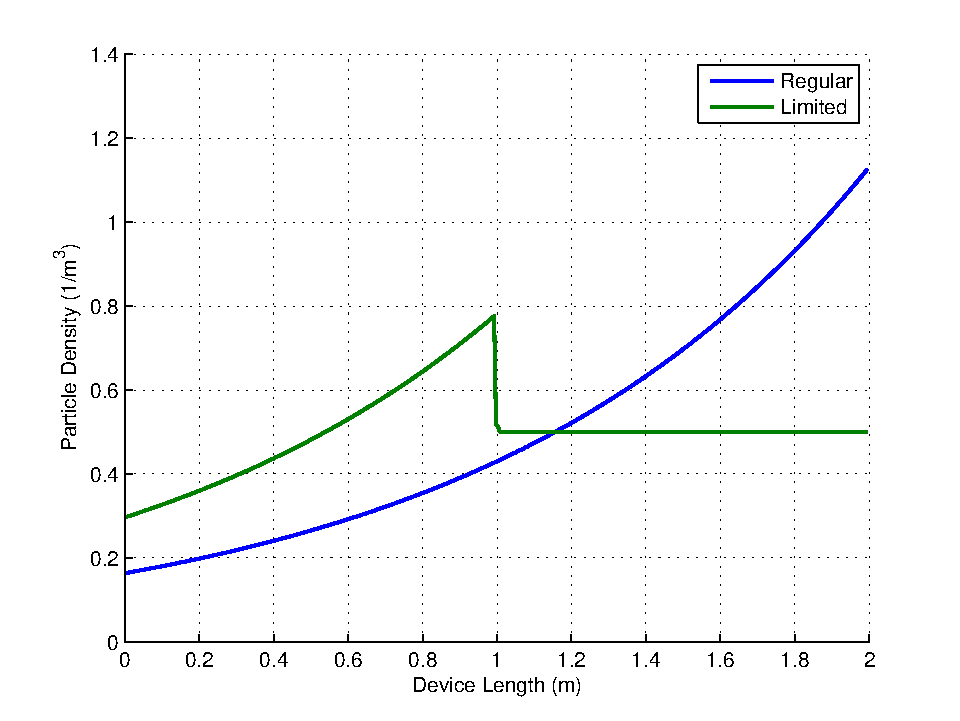
\includegraphics[scale=0.7]{5413}
\caption{Limited Density Accumulation on the Right Side} 
\label{5413}
\end{figure}

When the potential is switched all the particles accumulate freely at the left side of the simulation domain since there are no restrictions on this side (figure \ref{5414}).

\begin{figure}[!htp]
\centering
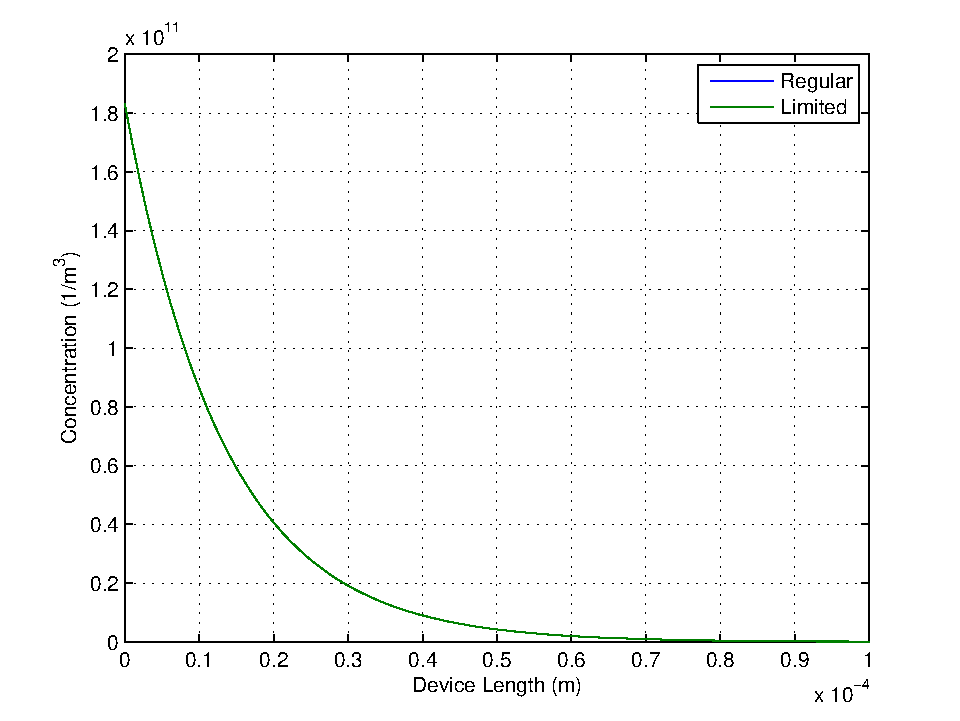
\includegraphics[scale=0.7]{5414}
\caption{Limited Concentration Density on the Left Side} 
\label{5414}
\end{figure}

This last figure (\ref{5411}) shows the transient response over time of a single node on the right side. The potential is positive for the first 1.5 seconds and it is switched to negative for the last 1.5 seconds. The node without any limit keeps accepting charge until a steady state has been reached but the density limited node stops accepting charged particles once the limit is reached. After the potential is switched density limited node has no problem releasing the particles.


\begin{figure}[!htp]
\centering
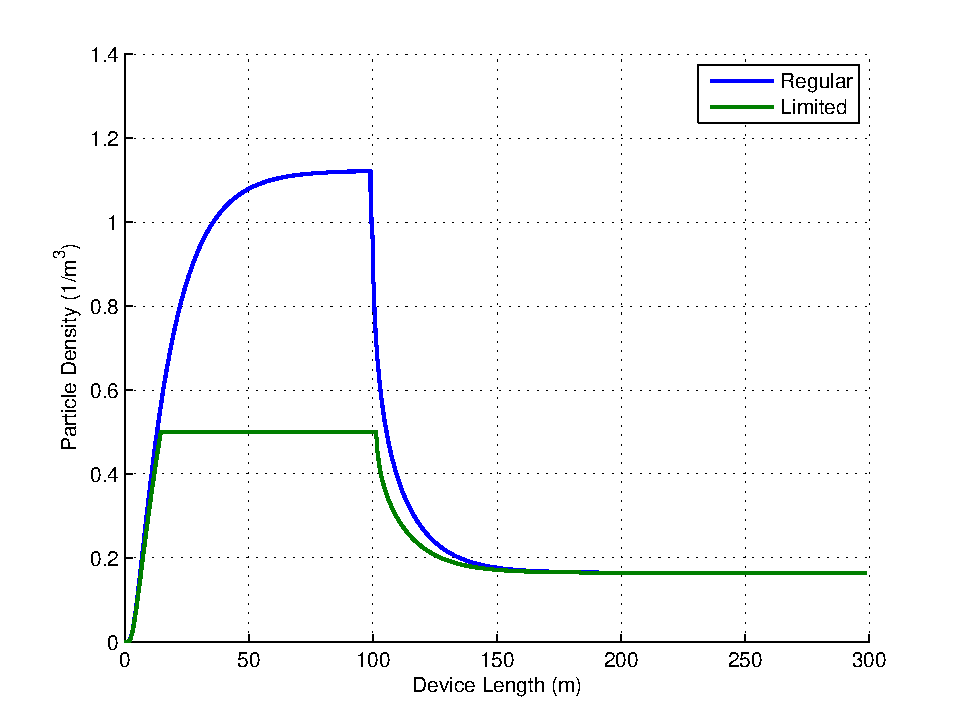
\includegraphics[scale=0.7]{5411}
\caption{Accumulation at the right wall over time} 
\label{5411}
\end{figure}

Additional to the test that is run for finite difference, COMSOL is used to test the soft limiting mechanism. COMSOL does not have a built in option that allows limiting the particle density. One possible solution to this is making particle mobility and diffusivity a function particle density. It is possible to use a sigmoid function which switches from 1 to 0 very quickly when particle density is close to its limit. Here is the equation of the sigmoid function used to limit the particle flow:

\begin{equation}
\mu_v = \frac{\mu_{0}}{1+e^{\sigma(n-n')}}
\label{mur}
\end{equation} 

$\mu_0$ is the original mobility of the charge carrier. $\sigma$ controls the slope of the switch and $n'$ determines the density at which the transition will be. 

Another problem with COMSOL is the definition of mobility and diffusion coefficients. When they are defined discontinuously and one of the mobilities is a function of the particle density like the example above, then COMSOL has convergence issues. To overcome the convergence problems, mobilities are set up to gradually switch from a constant value to a variable mobility using two more sigmoid functions which are dependent on position.

\begin{equation}
\mu=\frac{\mu_{v}}{1+e^{\sigma_x(x-x')}}+\frac{\mu_{c}}{1+e^{-\sigma_x(x-x')}}
\end{equation}

In this problem $\mu_v$ is the same as equation \ref{mur} since the region on the right side has a variable mobility and $\mu_c$ is just a constant mobility defined for the left side. $x'$ is the middle of the simulation area.

The initial carrier distribution for COMSOL is set to be exactly the same as finite difference simulation. Figures \ref{5416} and \ref{5423} show results for both COMSOL and finite difference simulations at steady state before the switch of the applied potential. The plot on the left side gives insight on how COMSOL simulation behaves for limited and limitless accumulation on the right wall. Due to the gradual change of mobility and diffusion constants between two areas, the density on the right side is higher than the limit which is $2 \; 10^{10}$. Additionally, the particle density goes over its limit near the right wall. In figure \ref{5423} the difference between COMSOL and finite difference becomes more visible. In FD simulation the accumulation goes much higher due to higher electric field and unlike COMSOL it does not penetrate the right half of the simulation domain. 

\begin{figure}[ht]
\centering
\begin{minipage}[b]{0.45\linewidth}
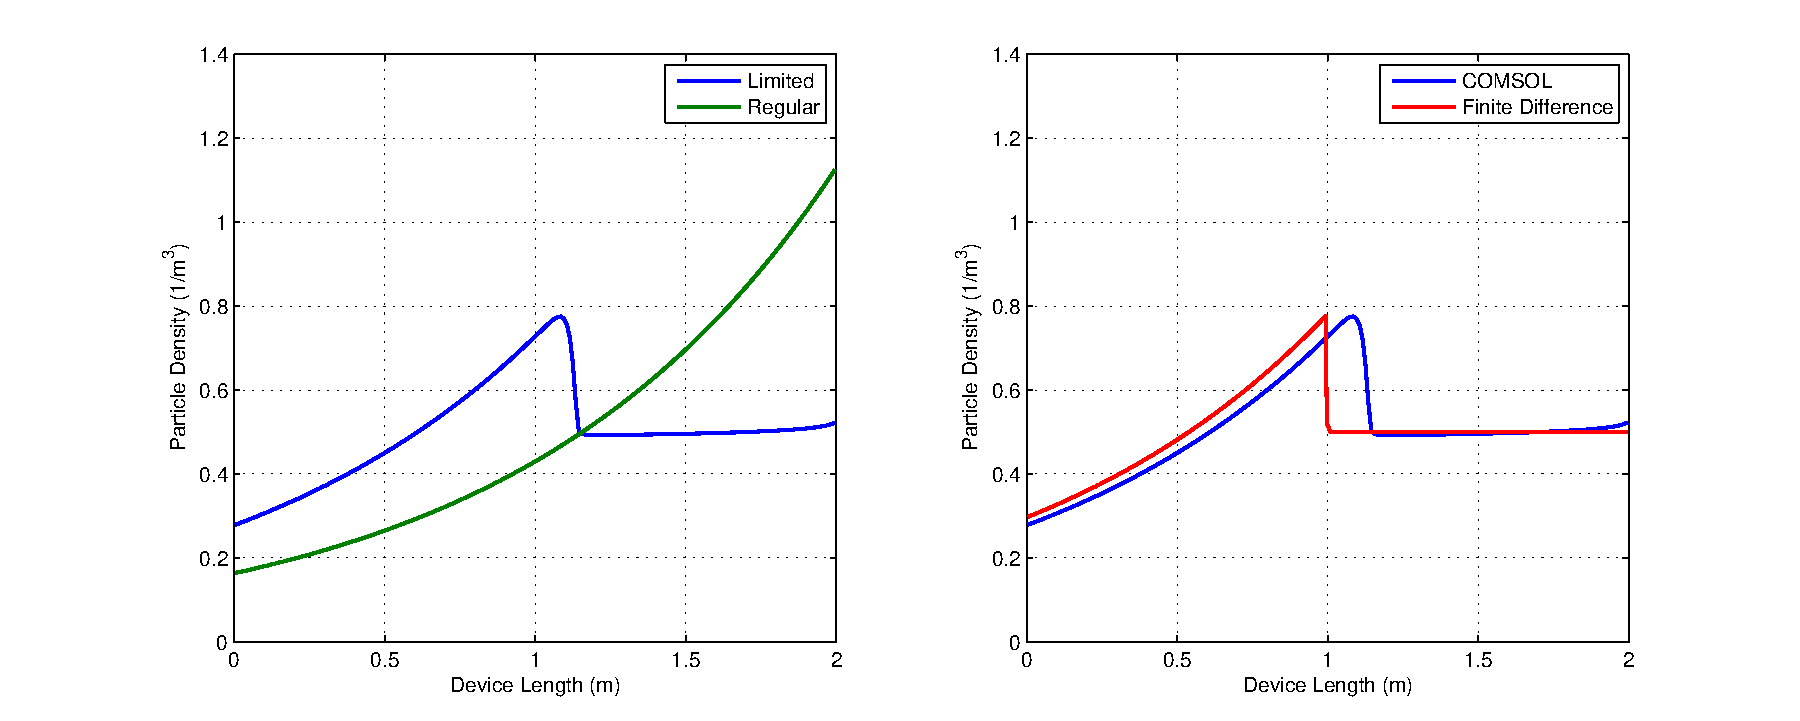
\includegraphics[scale=0.45]{5416}
\caption{COMSOL Simulation for Particle Density Limit}
\label{5416}
\end{minipage}
\quad
\begin{minipage}[b]{0.45\linewidth}
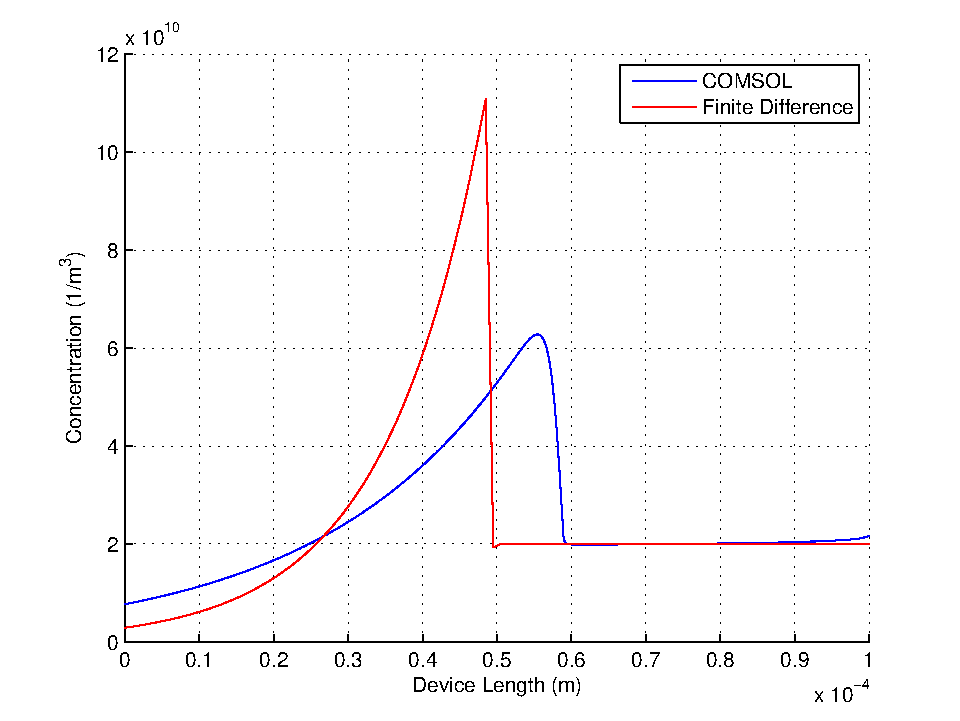
\includegraphics[scale=0.45]{5423}
\caption{COMSOL and Finite Difference Simulation}
\label{5423}
\end{minipage}
\end{figure}

In figure \ref{5417} it is possible to see the accumulation of charge near the middle section after the potential is switched. This is due to mobility being a function of distance and density. As the ions move from left to right they go from a low mobility region to a high mobility region and they slowly accumulate around the area where the change in mobility occurs. Figure comparing both COMSOL and finite difference shows that the accumulation does not happen in the case of finite difference due to the way density limiting mechanism is implemented.

\begin{figure}[ht]
\centering
\begin{minipage}[b]{0.45\linewidth}
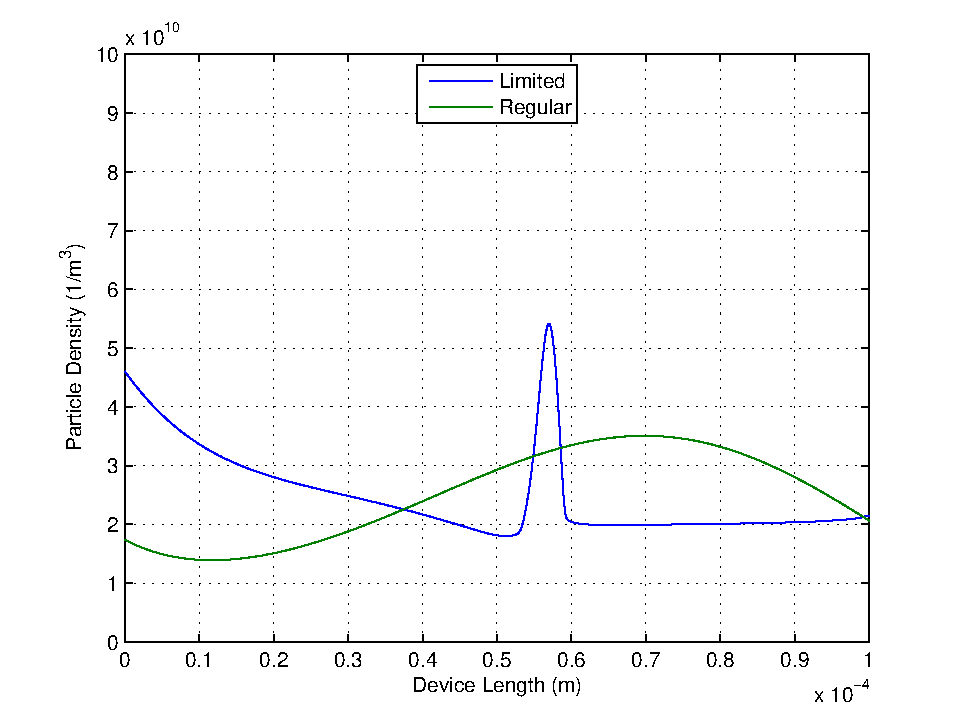
\includegraphics[scale=0.45]{5417}
\caption{COMSOL Simulation for Particle Density Limit}
\label{5417}
\end{minipage}
\quad
\begin{minipage}[b]{0.45\linewidth}
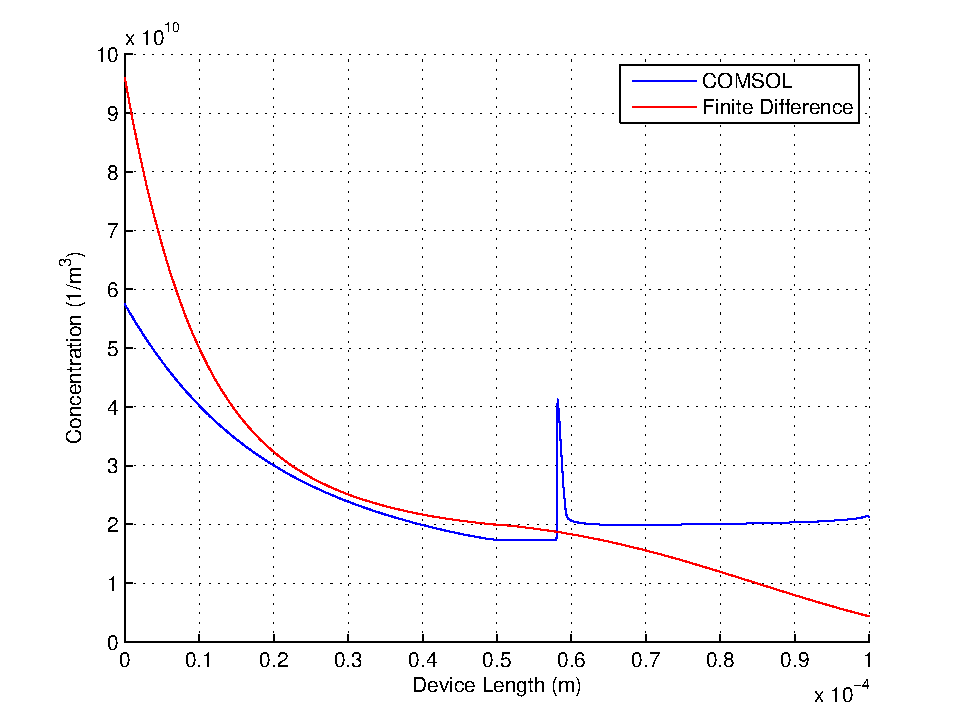
\includegraphics[scale=0.45]{5424}
\caption{COMSOL and Finite Difference Simulation}
\label{5424}
\end{minipage}
\end{figure}

With the decrease of ion density on the limited region the difference between low and high mobility regions diminish. Once the density on the limited side is low enough the whole system behaves as if there is no limit and ion mobility becomes equal for all regions and the ions freely accumulate on the left wall (figure \ref{5418}). Aside from the difference in electric field strength both simulations behave the same way as they approach steady state. Figure \ref{5426} shows densities at steady state. COMSOL simulation has a lower electric field since it has convergence issues with high electric fields. 

\begin{figure}[ht]
\centering
\begin{minipage}[b]{0.45\linewidth}
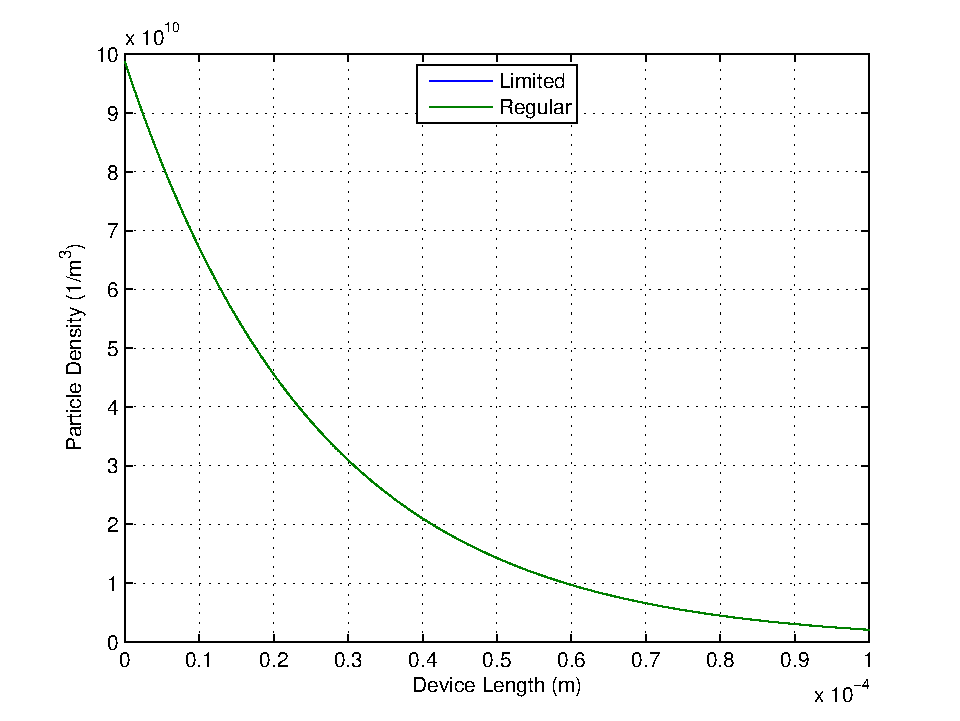
\includegraphics[scale=0.45]{5418}
\caption{COMSOL Simulation for Particle Density Limit}
\label{5418}
\end{minipage}
\quad
\begin{minipage}[b]{0.45\linewidth}
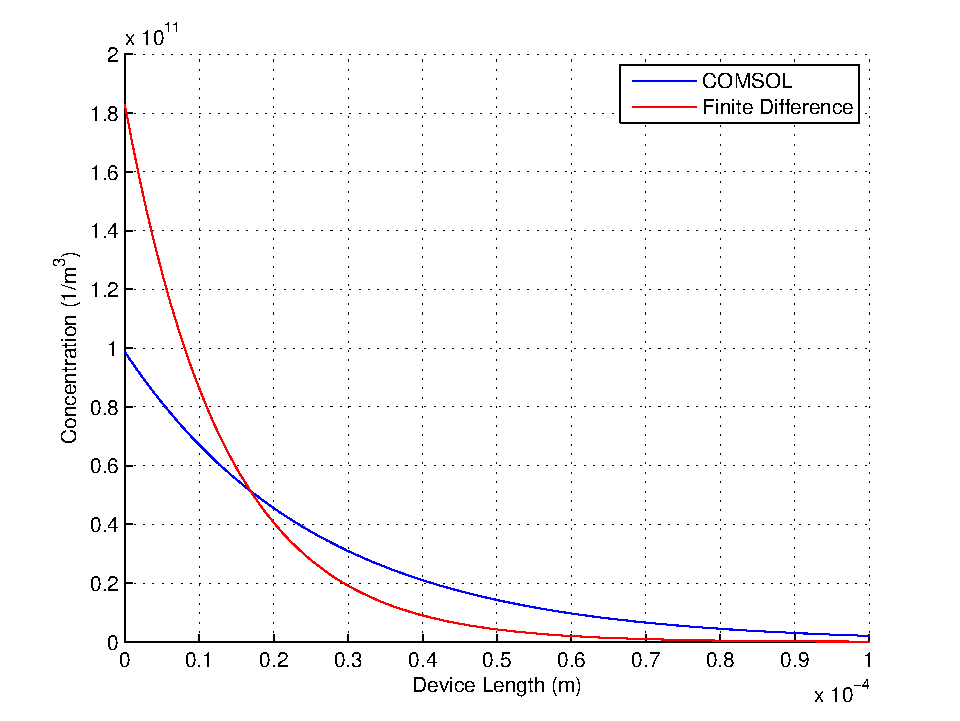
\includegraphics[scale=0.45]{5426}
\caption{COMSOL and Finite Difference Simulation}
\label{5426}
\end{minipage}
\end{figure}

This comparison can be finalized by looking the particle density transient response of the rightmost node. For the first half of the simulation everything is the same as the finite difference case except COMSOL goes a little bit over the limit. When the potential is switched, node without the limit has no noticeable difference in behaviour. The node with density limit has a lag when it comes to releasing the particles. This is due to the sigmoid function used to achieve a limiting behaviour. Once the limit is reached mobility and diffusivity are stuck at a very low value until the particle density starts to go lower than the limit.
\begin{figure}[ht]
\centering
\begin{minipage}[b]{0.45\linewidth}
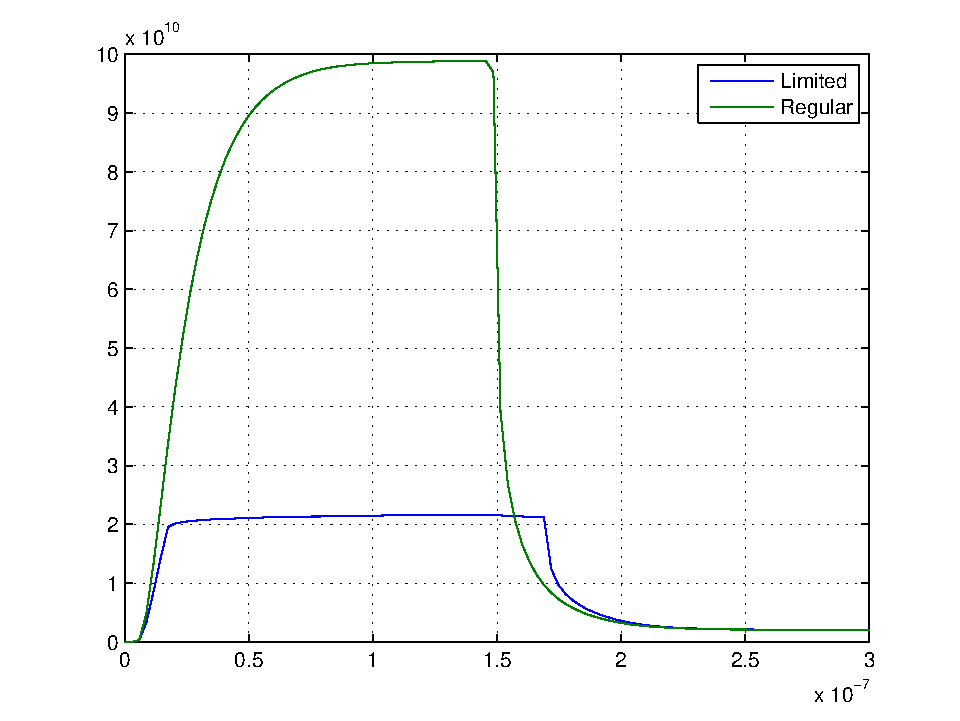
\includegraphics[scale=0.45]{5419}
\caption{Density on the right wall over time using COMSOL}
\label{5419}
\end{minipage}
\quad
\begin{minipage}[b]{0.45\linewidth}
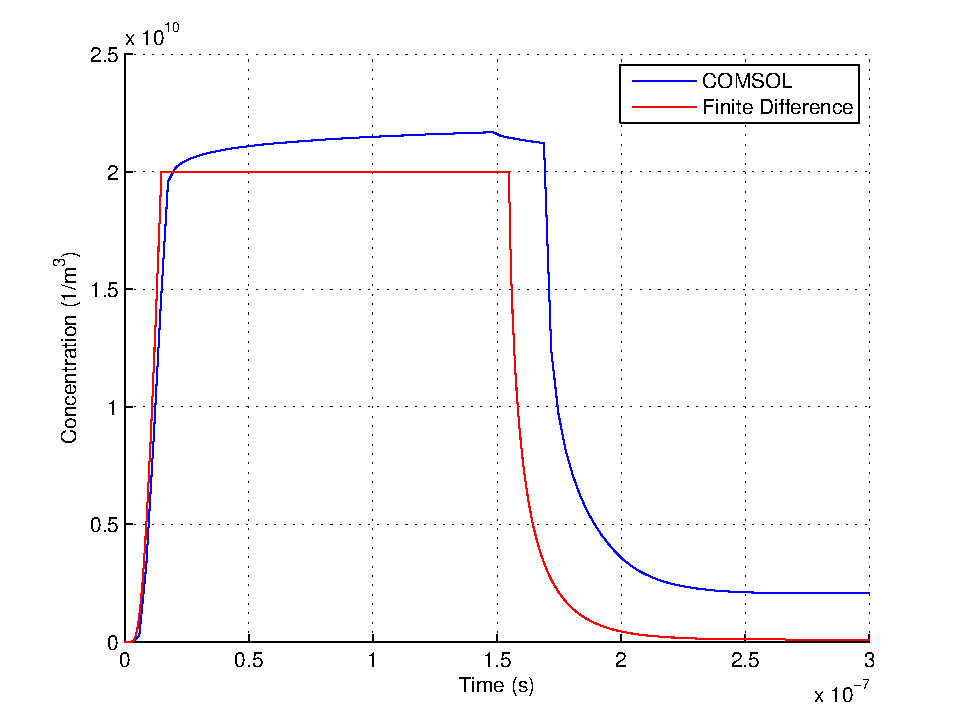
\includegraphics[scale=0.45]{5421}
\caption{Density on the right wall over time,COMSOL vs. Finite Difference}
\label{5421}
\end{minipage}
\end{figure}

The simulations above show that it is possible to impose a density limit over any area using a simple no flow boundary condition in a numerical simulation. For COMSOL some workarounds are implemented in order to simulate the same behavior without any convergence issues. 


\end{doublespace}